\subsection{Conway's Game of Life}

Invented by British mathematician John Horton Conway in 1970, Conway's Game of Life (or just ``Life''), has become iconic both within academia and elsewhere, and was thought to be a fitting demonstration of real-time graphics and game logic using Haskell. 

\begin{marginfigure}
	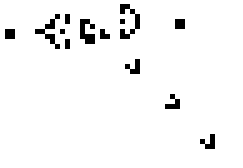
\includegraphics{res/conway/conway.png}
	\caption[Glider gun in Conway's Game of Life]{Glider gun in Conway's Game of Life.}
	\label{fig:glidergun}
\end{marginfigure}

Life is a basic example of a cellular automata. A rectangular grid of cells that can be either dead or alive is the game field, and each time step which cells are alive and which are dead are updated. The standard rules are a cell dies if it has fewer than 2 neighbours or more than 3, a dead cell comes to life if it has exactly three neighbours, otherwise the cells stay in their previous state.\sidenote{For more details on the Game of Life, see Gardner 1970, and \url{pentadecathlon.com/lifeNews/index.php}.}

The implementation starts with a paused grid of dead cells. The user can toggle the state of a cell by clicking it, and stop and start the simulation by pressing the space bar. Array data types from "Data.Array" are used to store the state of the game, and the topology is made to ``wrap around'' so events on the leftmost edge effect the right etc.

The logic and rules of the game of life were coded using pure code, and then the library \emph{Gloss} was used to draw the game board, update the board by calling the pure logical functions, and process mouse and keyboard events. The complete program is only 90 lines of Haskell.

\begin{marginfigure}
	\hspace{-1em}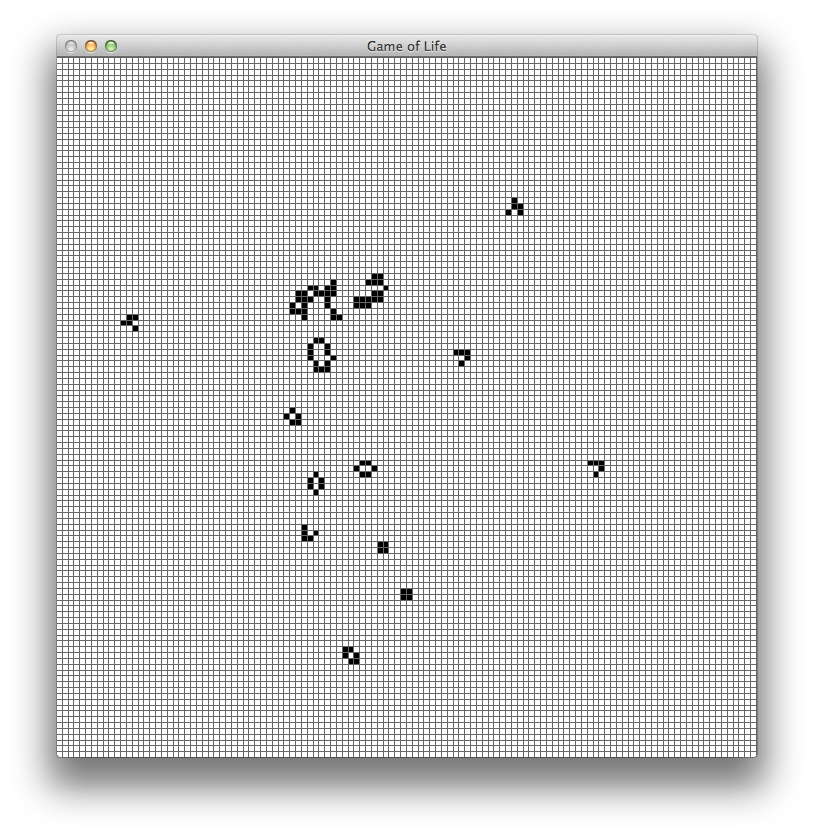
\includegraphics[width=18em]{res/conway/life.png}
	\caption[Full screen from Haskell implementation of life]{Full screen from Haskell implementation of life, showing gridlines.}
	\label{fig:life}
\end{marginfigure}

It was this experiment, and the ease of the implementation that led to the decision to use Gloss for the main game, as its simplicity would allow rapid development of an early version.